\documentclass[12pt]{article}
\usepackage{times} 			% use Times New Roman font

\usepackage[margin=1in]{geometry}   % sets 1 inch margins on all sides
\usepackage{hyperref}               % for URL formatting
\usepackage[pdftex]{graphicx}       % So includegraphics will work
\setlength{\parskip}{1em}           % skip 1em between paragraphs
\usepackage{indentfirst}            % indent the first line of each paragraph
\usepackage{datetime}
\usepackage[small, bf]{caption}
\usepackage{listings}               % for code listings
\usepackage{xcolor}                 % for styling code
\usepackage{multirow}

%New colors defined below
\definecolor{backcolour}{RGB}{246, 246, 246}   % 0xF6, 0xF6, 0xF6
\definecolor{codegreen}{RGB}{16, 124, 2}       % 0x10, 0x7C, 0x02
\definecolor{codepurple}{RGB}{170, 0, 217}     % 0xAA, 0x00, 0xD9
\definecolor{codered}{RGB}{154, 0, 18}         % 0x9A, 0x00, 0x12

%Code listing style named "gcolabstyle" - matches Google Colab
\lstdefinestyle{gcolabstyle}{
  basicstyle=\ttfamily\small,
  backgroundcolor=\color{backcolour},   
  commentstyle=\itshape\color{codegreen},
  keywordstyle=\color{codepurple},
  stringstyle=\color{codered},
  numberstyle=\ttfamily\footnotesize\color{darkgray}, 
  breakatwhitespace=false,         
  breaklines=true,                 
  captionpos=b,                    
  keepspaces=true,                 
  numbers=left,                    
  numbersep=5pt,                  
  showspaces=false,                
  showstringspaces=false,
  showtabs=false,                  
  tabsize=2
}

\lstset{style=gcolabstyle}      %set gcolabstyle code listing

% to make long URIs break nicely
\makeatletter
\g@addto@macro{\UrlBreaks}{\UrlOrds}
\makeatother

% for fancy page headings
\usepackage{fancyhdr}
\setlength{\headheight}{13.6pt} % to remove fancyhdr warning
\pagestyle{fancy}
\fancyhf{}
\rhead{\small \thepage}
\lhead{\small HW\#6, TOMAR}  % EDIT THIS, REPLACE # with HW number
\chead{\small CS 532, Spring 2023} 

%-------------------------------------------------------------------------
\begin{document}

\begin{centering}
{\large\textbf{HW\#6 - Analyzing Disinformation Domains }}\\ % EDIT THIS
                                % REPLACE # with HW num and ADD title
PRASHANT TOMAR\\                     % EDIT THIS
04/09/2023\\                      % EDIT THIS
\end{centering}

%-------------------------------------------------------------------------

\section*{Q1 - Data Analysis}

\subsection*{Answer}
To conduct this analysis, I created a python script that extracts the top 10 websites based on the number of tweets they have. Once the data is collected, I utilized the request library to assess the status of the website and check whether it is still operational.
\\
\begin{table}[h]
\centering
\caption{D1 analysis}
\label{tbl:simple}
\begin{tabular}{p{0.40\linewidth}p{0.20\linewidth}p{0.20\linewidth}p{0.15\linewidth}}
\hline
\textbf{Domains} & \textbf{Type} & \textbf{Tweets #} & \textbf{Status} \\ \hline \hline
\url{therealstrategy.com} & Alternative Media & 7113.0 & Live \\ \hline
\url{infowars.com} & Alternative Media & 1741.0 & Live \\ \hline
\url{newsbusters.org} & Alternative Media & 1217.0 & Live \\ \hline
\url{washingtonpost.com} & MSM & 1108.0 & Live \\ \hline
\url{nodisinfo.com} & Alternative Media & 774.0 & Not Live \\ \hline
\url{nytimes.com} & MSM & 759.0 & Live \\ \hline
\url{veteranstoday.com} & Alternative Media & 586.0 & Live \\ \hline
\url{beforeitsnews.com} & Alternative Media & 580.0 & Live \\ \hline
\url{rawstory.com} & Alternative Media & 308.0 & Live \\ \hline
\url{hoax.trendolizer.com} & fact checker & 299.0 & Live \\ \hline \hline

\end{tabular}
\end{table}


\\
\begin{table}[h]
\centering
\caption{D2 analysis}
\label{tbl:simple}
\begin{tabular}{p{0.40\linewidth}p{0.20\linewidth}p{0.20\linewidth}p{0.15\linewidth}}
\hline
\textbf{Domains} & \textbf{Type} & \textbf{Tweets #} & \textbf{Status} \\ \hline \hline
\url{21stcenturywire.com} & Blogging Site & 3088 & Not Live \\ \hline
\url{clarityofsignal.com} & Geopolitical Info & 2352 & Live \\ \hline
\url{rt.com} & News Channel & 1598 & Live \\ \hline
\url{newsweek.com} & Magazine site & 1249.0 & Not Live \\ \hline
\url{alternet.org} & Magazine & 1221 & Live \\ \hline
\url{sputniknews.com} & Newsfeed site & 1076.0 & Live \\ \hline
\url{mintpressnews.com} & Journalism & 919.0 & Not Live \\ \hline
\url{cnn.com} & News channel & 756.0 & Live \\ \hline
\url{globalresearch.ca} & research site & 724.0 & Live \\ \hline
\url{theantimedia.org} & News Channel & 682.0 & Live \\ \hline \hline

\end{tabular}
\end{table}

\clearpage

\begin{lstlisting}[language=Python, caption=Generate a graph for various cluster sizes.] 
import pandas as pd
from pandas import DataFrame
import requests

def check_website_status(domain):
    website_status = 'Live'
    try:
        response = requests.get('http://' + domain, timeout = 10)
        if response.status_code != 200:
            website_status = 'Not Live'
    except:
        website_status = 'Not Live'
    return website_status

# Implementation for D1
D1 = pd.read_csv('D1.csv')
D1 = D1.sort_values('# Citations in our Alternative Narrative Tweets', ascending=False)
D1 = D1.iloc[0:10, [0,1,4]]
D1_list = []

for index, row in D1.iterrows():
    website_status = check_website_status(row['Domain'])
    website_object = { 
        'domain': row['Domain'], 
        'type': row['Media Type (Determined through Content Analysis)'],
        'tweets': row['# Citations in our Alternative Narrative Tweets'],
        'status': website_status
        }

    D1_list.append(website_object)

D1_updated_dataframe = DataFrame(D1_list)
D1_updated_dataframe.to_csv('D1_updated_dataset.csv')

# Implementation for D2
D2 = pd.read_csv('D2.csv')
D2 = D2.sort_values('Tweet count', ascending=False)
D2 = D2.iloc[0:10, [0,2]]
D2_list = []

for index, row in D2.iterrows():
    website_status = check_website_status(row['Domain'])
    website_object = { 
        'domain': row['Domain'], 
        'type': '',
        'tweets': row['Tweet count'],
        'status': website_status
        }

    D2_list.append(website_object)

D2_updated_dataframe = DataFrame(D2_list)
D2_updated_dataframe.to_csv('D2_updated_dataset.csv')


\end{lstlisting}

\subsection*{Analysis}
To conduct the analysis, I opened each website in a browser and navigated to its "about us" page to determine its media type. The top shared tweets were mainly from large organizations such as cnn.com and rt.com. Upon further analysis, it was revealed that most of the domains were affiliated with news channels and independent blogging industries that commonly share news and critiques regarding governments and geopolitical information.

\clearpage

\section*{Q2 - Dataset Overlap}

\subsection*{Answer}
To obtain the unique domains from each dataset DataFrame and identify any overlapping domains between different datasets, I utilized the set feature in Python and employed the sets intersection method.

Result of these overlaps are shared below, 

\\
\begin{table}[h]
\centering
\caption{Dataset Combination}
\label{tbl:simple}
\begin{tabular}{p{0.25\linewidth}p{0.25\linewidth}}
\hline
\textbf{Dataset Combination} & \textbf{Count}  \\ \hline \hline
\url{D1 & D2 } & 36 \\ \hline
\url{D2 & D3 } & 21 \\ \hline
\url{D1 & D3 } & 12 \\ \hline
\url{D1 & D2 & D3} & 10  \\ \hline \hline

\end{tabular}
\end{table}
\\
The table below displays the domains associated with each dataset. To identify the unique links that belong to each dataset, I utilized a set and have listed them in the table.

\begin{table}[h]
\centering
\caption{Domains belongs to above dataset}
\label{tbl:simple}
\begin{tabular}{p{0.30\linewidth}p{0.30\linewidth}p{0.30\linewidth}}
ukcolumn.org	&	intellihub.com		&	ronpaulinstitute.org	\\ \hline
beforeitsnews.com	&	lewrockwell.com		&	theintercept.com	\\ \hline
off-guardian.org	&	blacklistednews.com		&	presstv.com	\\ \hline
foxnews.com	&	thefreethoughtproject.com		&	rt.com	\\ \hline
investmentwatchblog.com	&	theeventchronicle.com		&	themillenniumreport.com	\\ \hline
gellerreport.com	&	thewashingtonstandard.com		&	theguardian.com	\\ \hline
infowars.com	&	sott.net		&	21stcenturywire.com	\\ \hline
breitbart.com	&	nbcnews.com		&	collective-evolution.com	\\ \hline
fellowshipoftheminds.com	&	globalresearch.ca		&	cnn.com	\\ \hline
thestar.com	&	theantimedia.org		&	dailymail.co.uk	\\ \hline
nydailynews.com	&	thetruthseeker.co.uk		&	thedailysheeple.com	\\ \hline
abovetopsecret.com	&	theduran.com		&	nytimes.com	\\ \hline
rubikon.news	&	humansarefree.com		&		\\ \hline
thedailybeast.com	&	davidicke.com		&		\\ \hline
upi.com	&	dcclothesline.com		&		\\ \hline
wakingtimes.com	&	heavy.com		&		\\ \hline
activistpost.com	&	worldtruth.tv		&		\\ \hline

\end{tabular}
\end{table}


\clearpage
The following section contains the shared implementation of the dataset mentioned above.

\begin{lstlisting}[language=Python, caption=Generate a graph for various cluster sizes.] 
import pandas as pd
from pandas import DataFrame

def lowercase_domain_names(dataset):
    dataset["Domain"] = dataset["Domain"].str.lower()
    return dataset

def get_mutual_links(dataset1, dataset2):
    links_set1 = set(dataset1.iloc[:,0])
    links_set2 = set(dataset2.iloc[:,0])
    mutual_links = set.intersection(links_set1, links_set2)
    return mutual_links

def save_mutual_dataset(mutual_links, file_name):
    mutual_dataset = DataFrame(mutual_links, columns=['Domain'])
    mutual_dataset.to_csv(file_name, index=False)

def count_domains(file_name):
    mutual_dataset = pd.read_csv(file_name)
    count = len(mutual_dataset.index)
    return count

def get_unique_domains(*args):
    list_domains = []
    for file_name in args:
        mutual_dataset = pd.read_csv(file_name)
        for index, row in mutual_dataset.iterrows():
            list_domains.append(str(row['Domain']))
    domain_set = set(list_domains)
    unique_domains = list(domain_set)
    return unique_domains

# Lowercase domain names in all datasets
D1_dataset = pd.read_csv('D1.csv')
D1_dataset = lowercase_domain_names(D1_dataset)
D2_dataset = pd.read_csv('D2.csv')
D2_dataset = lowercase_domain_names(D2_dataset)
D3_dataset = pd.read_csv('D3.csv')
D3_dataset = lowercase_domain_names(D3_dataset)

# Find mutual links between datasets
D1_D2_mutual_links = get_mutual_links(D1_dataset, D2_dataset)
D2_D3_mutual_links = get_mutual_links(D2_dataset, D3_dataset)
D1_D3_mutual_links = get_mutual_links(D1_dataset, D3_dataset)
D1_D2_D3_mutual_links = set.intersection(D1_D2_mutual_links, D3_dataset.iloc[:,0])

# Save mutual datasets to CSV files
save_mutual_dataset(D1_D2_mutual_links, 'D1_D2_mutual_links.csv')
save_mutual_dataset(D2_D3_mutual_links, 'D2_D3_mutual_links.csv')
save_mutual_dataset(D1_D3_mutual_links, 'D1_D3_mutual_links.csv')
save_mutual_dataset(D1_D2_D3_mutual_links, 'D1_D2_D3_mutual_links.csv')

# Count number of domains in each mutual dataset
D1_D2_mutual_count = count_domains('D1_D2_mutual_links.csv')
D2_D3_mutual_count = count_domains('D2_D3_mutual_links.csv')
D1_D3_mutual_count = count_domains('D1_D3_mutual_links.csv')
D1_D2_D3_mutual_count = count_domains('D1_D2_D3_mutual_links.csv')

# Print unique domains
unique_domains = get_unique_domains('D1_D2_mutual_links.csv', 'D2_D3_mutual_links.csv', 'D1_D3_mutual_links.csv', 'D1_D2_D3_mutual_links.csv')
for domain in unique_domains:
    print(domain)

\end{lstlisting}

\subsection*{Analysis}

An interesting observation about the list of mutual domains is that all of the website domains included are highly popular.
 
\clearpage

\section*{Q3 - Disinformation Games}

\subsection*{Answer}

I played the game on https://goviralgame.com and found it to be an engaging and informative experience. The game is designed to educate players about how disinformation spreads on social media platforms, and it does this by putting the player in the shoes of someone creating and spreading fake news. Through a series of choices and actions, the player can choose to create fake news articles, purchase bots to spread the articles, and use other tactics to increase their reach.

As I played the game, I found myself becoming more and more aware of the tactics used by people who create and spread fake news. I learned about the importance of verifying sources, fact-checking information before sharing it, and being critical of sensational headlines. The game also emphasized the importance of responsible social media use and how our actions online can have real-world consequences.

Overall, I found the game to be a thought-provoking and engaging way to learn about the dangers of disinformation. The game's design and user interface were easy to navigate, and the graphics were well-done. I appreciated the opportunity to experience the creation and spread of disinformation in a safe and controlled environment and would recommend this game to anyone looking to learn more about the topic. Below are some screenshots from my playthrough:


\begin{figure}[h]
\caption{Final result of Game}
\centering
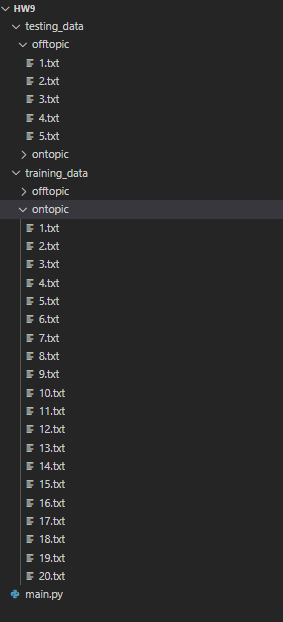
\includegraphics[width=\textwidth]{pic1.png}
\end{figure}
 
\clearpage


\section*{References}



\begin{itemize}
    \item {Bar charts seaborn library, \url{https://seaborn.pydata.org/generated/seaborn.barplot.html}}
    \item {DataFrame operations, \url{https://pandas.pydata.org/docs/reference/api/pandas.DataFrame.groupby.html}}
    \item {Tweepy, \url{https://docs.tweepy.org/en/latest/}}
    \item {Numpy, \url{https://numpy.org/doc/stable/reference/generated/numpy.log2.html}}
    \item {Goviralgame, \url{https://www.goviralgame.com/en/play}}
    \item {Github Datasets, \url{https://github.com/odu-cs432-websci/spring23-hw6-Badjedi04}}
    
\end{itemize}

\end{document}
